\documentclass[11pt,letterpaper]{article}
\usepackage{../packageslc}
\usepackage{../optionslc}
\usetikzlibrary{matrix}

%%%% Macros para las notas de lenguajes de programacion


%%%% math

\newcommand{\vphi}{\varphi}
\newcommand{\vp}{\varphi}

% \newcommand{\dn}{\mathsf{DN}}
% \newcommand{\dnC}{\mathsf{DN_C}}
% \newcommand{\dnM}{\mathsf{DN_M}}
% \newcommand{\dnp}{\mathsf{DN_p}}
% \newcommand{\dnm}{\mathsf{DN_p^M}}
% \newcommand{\dnc}{\mathsf{DN_p^C}}

%\newcommand{\case}{\mathsf{case}}
%\renewcommand\labelitemi{$\circ$}

\newcommand{\imp}{\rightarrow}
\newcommand{\Imp}{\Rightarrow}
\renewcommand{\iff}{\leftrightarrow}
\newcommand{\Iff}{\Leftrightarrow}
\newcommand{\G}{\Gamma}
\newcommand{\D}{\Delta}


\newcommand{\De}{\mathcal{D}}
\newcommand{\F}{\mathcal{F}}
\newcommand{\Ge}{\mathcal{G}}
\newcommand{\Pe}{\mathcal{P}}
\newcommand{\I}{\mathcal{I}}
\newcommand{\C}{\mathcal{C}}
\newcommand{\K}{\mathcal{K}}
\renewcommand{\L}{\mathcal{L}}
\newcommand{\M}{\mathcal{M}}
\newcommand{\Nc}{\mathcal{N}}
%\newcommand{\E}{\mathcal{E}}
%\newcommand{\R}{\mathcal{R}}
%\newcommand{\Q}{\mathcal{Q}}
\newcommand{\Sc}{\mathcal{S}}
\newcommand{\Te}{\mathcal{T}}
\newcommand{\W}{\mathcal{W}}

\newcommand{\Db}{\mathbb{D}}
\newcommand{\Fb}{\mathbb{F}}
\newcommand{\Kb}{\mathbb{K}}
\newcommand{\Eb}{\mathbb{E}}
\newcommand{\Ebs}{\mathbb{E}^\star}
\newcommand{\Ob}{\mathbb{O}}
\newcommand{\Ib}{\mathbb{I}}
\newcommand{\Rb}{\mathbb{R}}
\newcommand{\Qb}{\mathbb{Q}}
\newcommand{\Kbb}{\mathbb{K}}
\newcommand{\T}{\mathbb{\Theta}}


\newcommand{\kb}{\bbkappa}

\newcommand{\Sf}{\mathsf{\Sigma}}

\newcommand{\fa}{\forall}
\newcommand{\ex}{\exists}

\newcommand{\inc}{\subseteq}

\newcommand{\Lb}{\Lambda}
\newcommand{\Om}{\Omega}
\newcommand{\lb}{\lambda}
\newcommand{\al}{\alpha}
\newcommand{\ga}{\gamma}


\newcommand{\mg}{\mathbb{m}}

\newcommand{\cg}{\mathbb{C}}
\newcommand{\dg}{\mathbb{D}}
\newcommand{\jg}{\mathbb{J}}
\newcommand{\Ha}{\mathcal{H}}
%\newcommand{\A}{\mathcal{A}}
\newcommand{\sg}{\mathbb{S}}

\newcommand{\Bc}{\mathcal{B}}
\newcommand{\Df}{\mathfrak{D}}
\newcommand{\Dc}{\mathcal{D}}
%\newcommand{\Tc}{\mathcal{T}}
\newcommand{\Mf}{\mathfrak{M}}

\newcommand{\Sg}{\mathbb{S}}

\newcommand{\Q}{\ensuremath{\mathbb{Q}}}
\newcommand{\Z}{\ensuremath{\mathbb{Z}}}
\newcommand{\N}{\ensuremath{\mathbb{N}}}
\newcommand{\R}{\ensuremath{\mathbb{R}}}
\renewcommand{\S}{\mathbb{\Sigma}}
\newcommand{\A}{\mathcal{A}}
\newcommand{\E}{\ensuremath{\exists}}
\newcommand{\iso}{\ensuremath{\cong}}
\newcommand{\union}{\ensuremath{\cup}}
\newcommand{\morinyec}{\ensuremath{\precapprox}}

\newcommand{\nin}{\ensuremath{\notin}}
\newcommand{\tog}{\makebox[7mm][l]}
\newcommand{\toge}{\makebox[11mm][l]}
\newcommand{\toget}{\makebox[13mm][l]}
\newcommand{\togeth}{\makebox[14mm][l]}
\newcommand{\togethe}{\makebox[15mm][l]}
\newcommand{\together}{\makebox[17mm][l]}
\newcommand{\niso}{\ensuremath{\not \cong}}


\newcommand{\Mg}{\mathbb{M}}
\newcommand{\Bg}{\mathbb{B}}
\newcommand{\Lg}{\mathbb{L}}
\newcommand{\Tg}{\mathbb{T}}

\newcommand{\sketch}{\Red{{\sc sketch}}}

\newcommand{\restr}[2]{#1\!\!\boldsymbol{\restriction}\!#2}

\newcommand{\vacio}{\varnothing}
\newcommand{\done}{\ensuremath{\checkmark}}

\newcommand{\ida}{$\Rightarrow \; )$ }
\newcommand{\regr}{$\Leftarrow \; )$ }

\newcommand{\ol}[1]{\overline{#1}}

\newcommand{\Tsf}{\mathsf{T}}

\newcommand{\inds}[1]{\index[simb]{#1}}

\newcommand{\B}{\mathbb{B}}
%\newcommand{\N}{\mathbb{N}}

\newcommand{\vx}{\vec{x}}
\newcommand{\vy}{\vec{y}}
\newcommand{\vz}{\vec{z}}
\newcommand{\vt}{\vec{t}}
\newcommand{\vf}{\vec{f}}


% \newcommand{\propo}{\ensuremath{\mathsf{PROP}}}
% \newcommand{\atom}{\ensuremath{\mathsf{ATOM}}}
\newcommand{\term}{\ensuremath{\mathsf{TERM}}}
\newcommand{\form}{\mathsf{FORM}}

\newcommand{\true}{\mathop{\mathsf{true}}}

%\newcommand{\id}{\mathsf{Id}}

%\newcommand{\uc}{\mathcal{U}}
%\newcommand{\Ic}{\mathcal{I}}
%\newcommand{\pc}{\mathcal{P}}
%\newcommand{\qc}{\mathcal{Q}}
%\newcommand{\mc}{\mathcal{M}}
\newcommand{\supc}{\supseteq}
\newcommand{\limo}{\mathop{\mathpzc{Lim}}}
\newcommand{\ord}{\mathsf{OR}}

\newcommand{\pt}[1]{\langle #1 \rangle}


%%%% frames
\newcommand{\titulos}[2]{\frametitle{#1}\framesubtitle{#2}}
\newcommand{\fot}[1]{\footnote{\scriptsize{#1}}}


%%%% ambientes

\newcommand{\cb}[2]{\colorbox{#1}{#2}}

\newcommand{\bc}{\begin{center}}
\newcommand{\ec}{\end{center}}
\newcommand{\be}{\begin{enumerate}}
\newcommand{\ee}{\end{enumerate}}
\newcommand{\bi}{\begin{itemize}}
\newcommand{\ei}{\end{itemize}}
\newcommand{\beq}{\begin{equation}}
\newcommand{\eeq}{\end{equation}}
\newcommand{\beqs}{\begin{equation*}}
\newcommand{\eeqs}{\end{equation*}}
\newcommand{\ba}{\begin{array}}
\newcommand{\ea}{\end{array}}


% \newtheorem{theorem}{Teorema}
% \newcommand{\teo}[1]{\begin{theorem} #1 \end{theorem}}
% \newtheorem{proposition}{Proposici\'on}
% \newcommand{\prop}[1]{\begin{proposition} #1 \end{proposition}}
% \newtheorem{definition}{Definici\'on}
% \newcommand{\defin}[1]{\begin{definition} #1 \end{definition}}
% \newtheorem{corollary}{Corolario}
% \newcommand{\cor}[1]{\begin{corollary} #1 \end{corollary}}
% \newtheorem{lemma}{Lema}
% \newcommand{\lema}[1]{\begin{lemma} #1 \end{lemma}}
% \newcommand{\dem}[1]{\begin{proof} #1 \end{proof}}

%\renewcommand{\qed}{\qedsymbol{$\mathbf{\dashv}$}}

%\newcommand{\proof}{\hfill\\\noindent\textbf{\textit{Demostraci\'on. }}}

\newcommand{\hint}{\emph{Sugerencia: }}


\newcounter{EjempCtr}[section]
\newenvironment{enumrom}{\renewcommand{\theenumi}{\roman{enumi}}%
\renewcommand{\theenumii}{\roman{enumii}}
\renewcommand{\theenumiii}{\roman{enumiii}}
\renewcommand{\theenumiv}{\roman{enumiv}}
\begin{enumerate}}{\end{enumerate}}
\newenvironment{Ejemplo}
        {\stepcounter{EjempCtr}%
        \begin{description}\item[Ejemplo \thesection.\arabic{EjempCtr}]}%
        {\end{description}}
\newenvironment{demostr}{%
             {\em Demostración:}
                \begin{quotation}}{\end{quotation}}

   \newcommand{\beje}{\begin{Ejemplo}}
\newcommand{\eeje}{\end{Ejemplo}}


\newtheorem{eje}{Ejemplo}[section]
\newcommand{\ejem}[1]{\begin{eje}\normalfont #1 \end{eje}}

% \renewcommand\contentsname{\'Indice}
%\renewcommand\chaptername{Cap\'itulo}
% \renewcommand\indexname{\'Indice}

%%\newcommand{\qed}{\hfill$\mathbb{Qed}$}
%\newcommand{\qed}{\hfill$\mathsf{\boldsymbol{\dashv}}$}
%\renewcommand{\qed}{\hfill$\boldsymbol{\dashv}$}


\newenvironment{prueba}{\vspace{-5mm}\noindent\textbf{Demostraci\'on}\\}{
\noindent$\blacksquare$\\}

\newcommand{\Ejercicios}{\section*{Ejercicios}}

 \newenvironment{manitas}{%
      \renewcommand{\labelitemi}{\ding{44}}%
      \vspace{-0.5cm}%
      \begin{itemize}%
      \setlength{\itemsep}{0pt}\setlength{\parsep}{0pt}\setlength{\topsep}{0pt}%
      }{\end{itemize}}
\newenvironment{malitos}{%
      \renewcommand{\labelitemi}%
            {\raisebox{1.5ex}{\makebox[0.3cm][l]{\begin{rotate}{-90}%
            \ding{43}\end{rotate}}}}%
      \vspace{-0.5cm}%
      \begin{itemize}%
      \setlength{\itemsep}{0pt}\setlength{\parsep}{0pt}\setlength{\topsep}{0pt}%
      }{\end{itemize}}
\newenvironment{ejercs}{
     \renewcommand{\labelenumi}{\thesection.\theenumi.-}
     \renewcommand{\labelenumii}{\theenumii)}
     \begin{enumerate}}
     {\end{enumerate}}

   \newcommand{\bej}{\begin{ejercs}}
\newcommand{\eej}{\end{ejercs}}


%\newenvironment{leterize}{%
%        \renewcommand{\theenumi}{\alph{enumi}}
%        \begin{enumerate}}{\end{enumerate}}

%\newenvironment{manitas}{%
%      \renewcommand{\labelitemi}{\ding{44}}%
%      \vspace{-0.5cm}%
%      \begin{itemize}%
%      
% \setlength{\itemsep}{0pt}\setlength{\parsep}{0pt}\setlength{\topsep}{0pt}%
%      }{\end{itemize}}



%%=============================================================================

\def\stackunder#1#2{\mathrel{\mathop{#2}\limits_{#1}}}


%%%% notas

\newcommand{\doubt}{\Red{{\LARGE {\sf ??}}}}

\newcommand{\coment}[1]{\hfill\\ \Big[{\bf Comentario Privado:} #1\Big]}
\newcommand{\preg}[1]{\hfill\\ \BrickRed{{\bf Pregunta:} #1}}
\newcommand{\conjet}[1]{\hfill\\ \OliveGreen{{\bf Conjecura:} #1}}

\newcommand{\pendiente}{\BrickRed{{\sc Pendiente}}}
\newcommand{\verifpendiente}{\BrickRed{{\sc Verificación pendiente}}}


%--------------------------------------------------------------------------

\DeclareMathAlphabet{\mathpzc}{OT1}{pzc}{m}{it}


\title{Lógica Computacional 2018-2, nota de clase 11 \\
Resolución binaria, fundamentos de programación lógica y {\pl}
}
\author{Favio Ezequiel Miranda Perea \and Araceli Liliana Reyes Cabello\and
Lourdes Del Carmen Gonz\'alez Huesca \and Pilar Selene Linares Arévalo}
\date{26 de abril de 2018 \\
Material desarrollado bajo el proyecto UNAM-PAPIME PE102117}
\begin{document}
\maketitle


\section{Resolución binaria con unificación}

La regla de resolución binaria es de primordial importancia para los sistemas
de programación lógica y razonamiento automatizado, al proporcionar un método
mecánico para decidir la consecuencia lógica $\G\vdash \vp$, mediante la
obtención de la cláusula vacía $\square$ a partir 
de las formas clausulares de las fórmulas del conjunto $\G\cup\{\lnot\vp\}$.


La regla de resolución para la lógica de predicados toma como
premisas dos cláusulas $\C,\De$ con variables ajenas tales que existe una
literal~$\ell$ en una de ellas y una literal $\ell'$ en la otra de manera que 
$\ell^c$ y $\ell'$ son \textbf{unificables} mediante un $\sigma$. 
La regla devuelve como conclusión la disyunción de las literales de $\C,\De$ 
después de eliminar las literales contrarias $\ell\sigma$ y $\ell'\sigma$, pero 
aplicando a cada una de ellas el unificador $\sigma$.

Esquemáticamente tenemos lo siguiente:
\begin{mathpar}
 \inferrule*[]{
 \C=_{def}\C_1\lor \ell \and \De=_{def}\De_1\lor \ell' \and
  Var(\C)\cap Var(\De)=\vacio \and\sigma\text{ umg de } \{\ell^c,\ell'\}
 }{
 (\C_1\lor\De_1)\sigma
 }
\end{mathpar}
En tal caso decimos que $(\C_1\lor\De_1)\sigma$ es un \textbf{resolvente} de
$\C$ y $\De$.\\
Obsérvese que la restricción acerca de las variables siempre puede obtenerse
al renombrar las variables de alguna de las cláusulas, lo cual es válido pues
las variables de una cláusula en realidad estaban cuantificadas
universalmente en una forma normal de Skolem.


\noindent Veamos un ejemplo
\begin{mathpar}
 \inferrule*[]{
 \C=Pxy\lor \neg Qax\and \De=Rz\lor Qzb
 }{
 Pby\lor Ra
 }
\end{mathpar}
en tal caso $\ell=\neg Qax,\;\ell'=Qzb$ y $\sigma=[x:=b,z:=a]$.


\medskip

\noindent Veamos ahora un ejemplo de decisión de consecuencia lógica utilizando 
resoluci\'on binaria:
\ejem{Verificar que 
$\fa x\ex y\big(Cx\imp Py\land Axy\big)\models 
  \fa z\big(Cz\imp\ex w(Pw\land Azw)\big)$.\\
La transformación a formas clausulares de la premisa y la negación de la
conclusión resulta en el siguiente conjunto:
\[
\{\neg Cx\lor Pfx,\;\neg Cx\lor Axfx,\;Ca,\;\neg Pw\lor\neg Aaw\}
\]
La derivación mediante resolución es:
\[
\begin{array}{rlc}
 1. & \neg Cx\lor Pfx & Hip. \\
 2. & \neg Cx\lor Axfx & Hip. \\
 3. & Ca & Hip. \\
 4. & \neg Pw\lor\neg Aaw & Hip. \\
 5. & Pfa & Res(1,3,[x:=a]) \\
 6. & \neg Aafa & Res(5,4,[w:=fa]) \\
 7. & \neg Ca & Res(6,2,[x:=a])\\
 8. & \cv & Res(3,7,\vacio)
\end{array}
\]
Dado que la cláusula vacía fue obtenida podemos concluir que la consecuencia
lógica original es válida.
}

Es importante mencionar que la restricción acerca de que las variables de las 
dos cláusulas sobre las que se va a aplicar la resolución sean ajenas es 
primordial para demostrar la completud refutacional, sin tal restricción 
tendr\'iamos por ejemplo que el conjunto insatisfacible 
$\{\fa x Px,\fa x \neg Pfx\}$  cuyas formas clausulares son $\{Px,\neg Pfx\}$, 
no permite derivar la cláusula vacía, pues el conjunto $\{Px,Pfx\}$ no es 
unificable.\\
El renombre de variables nos lleva al conjunto $\{Py,Pfx\}$ unificable
mediante $\sigma=[y:=fx]$.

\subsection{Correctud y completud refutacional}

Justificamos el método de semidecisión mediante resolución binaria con los 
teoremas correspondientes de correctud y completud. \\

Dado un conjunto de cláusulas~$\G$ y una cláusula~$\C$ decimos que $\C$ es
derivable a partir de $\G$ mediante resolución, y escribimos en tal caso
$\G\vdash_\mathcal{R}\C$, si $\C$ se obtuvo a partir de $\G$ usando
resolución binaria y equivalencias simplificativas (eliminación de literales
repetidas bajo unificación, proceso llamado factorización). \\
En el ejemplo anterior tenemos en particular $\G\vdash_\mathcal{R} \neg Ca$, 
donde $\G$ consta de las cláusulas 1 a 4.

\teo{[Correctud de la Resolución]
Si $\G\vdash_\mathcal{R}\C$ entonces $\G\models\C$.
}
\proof 
Basta observar que la regla de resolución preserva validez.
\qed

\medskip

Aquí la consecuencia lógica realmente significa $\fa\G\models\fa\C$, es decir
se restauran las formas normales de Skolem usando las cerraduras universales de 
las f\'ormulas. \\
Como corolario obtenemos la correctud refutacional:
\cor{[Correctud Refutacional de la Resolución] Si
  $\G\vdash_\mathcal{R}\square$ entonces $\G$ es insatisfacible.
}

Este corolario es el que permite que funcione el método del ejemplo anterior.
El recíproco de este teorema, llamado completud refutacional también es
cierto, aunque su demostración es compleja y no se abordar\'a en este curso.

\teo{[Completud Refutacional de la Resolución] 
Si $\G$ es insatisfacible entonces existe una derivación de la cláusula vacía
$\G\vdash_\mathcal{R}\square$.
}


\section{Breve introducción a la programación lógica}

Los lenguajes de programación más ampliamente usados, como {\sc C} o 
{\sc Java}, forman parte del paradigma de programación imperativa o 
procedimental cuyas características principales son:
\bi
 \item Un programa es una secuencia de instrucciones.
 \item La principal estructura de control son los ciclos:
  \emph{while, repeat, for} etc.
 \item La operación de asignación $x:=a$ es imprescindible.
 \item Las estructuras de control permiten seguir paso a paso las
   acciones que debe realizar un programa.
 \item Es decir, el programa especifica \emph{cómo} se calculan los resultados.
\ei
En contraste los lenguajes de programación funcional ({\sc Haskell, Lisp, 
Scheme, ML}) y lógica ({\pl}) conforman la llamada programación 
declarativa cuyas características principales son:
\bi
 \item Un programa es una sucesión de definiciones.
 \item La principal estructura de control es la recursión.
 \item No existen ni ciclos ni operación de asignación 
 \item El programa especifica \emph{qu\'e} se debe calcular, es decir, las
  propiedades que debe cumplir el resultado o solución a calcular.
 \item El \emph{c\'omo} es irrelevante.
\ei


\subsection{Ventajas de la programación declarativa}

La programación declarativa no depende del lenguaje en particular. 
\bi
 \item Si bien los programas imperativos pueden ser rápidos y especializados, un programa declarativo es más general, corto y legible. 
 \item Debido a lo anterior podemos decir que los programas declarativos son 
elegantes matemáticamente. Lo cual implica que es más fácil \textit{verificar} 
si el programa cumple su especificación.
 \item Aprender programación declarativa permite al programador desarrollar un 
estilo de programación riguroso y disciplinado  que puede ser usado 
ventajosamente sin importar el lenguaje de programación utilizado.
 \item Este estilo genera programas con una mejor ingenieria, más f\'aciles de 
depurar, mantener y modificar.
\ei


\subsection{Lenguajes de programación lógica}
%%%%% Del libro de Maribel Fernandez: Modelos de Computo

Fue alrededor de las d\'ecadas de 1920 y 1930 que Jacques 
Herbrand~\footnote{Jacques Herbrand (1908-1931), l\'ogico prominente que 
muri\'o a la edad de 23 años en un accidente en los alpes.} propuso en 
su tesis un m\'etodo para verificar la validez de f\'ormulas en l\'ogica de 
predicados utilizando un procedimiento para unificar f\'ormulas. \\
Esta tesis es el fundamento de la programaci\'on l\'ogica que modela al 
c\'omputo a trav\'es de los llamados modelos de Herbrand donde:
\be
\item el dominio es el universo formado por t\'erminos que representan objetos
\item las f\'ormulas que involucran predicados describen un problema
\ee

Las f\'ormulas son usadas para expresar conocimiento, en particular, 
descripciones o algoritmos en forma de funciones parciales creando un programa 
l\'ogico.
% que como vimos es un conjunto de cl\'ausulas.

Realizar c\'omputos a partir de un programa l\'ogico es obtener respuestas a 
partir de la informaci\'on descrita. 
Las respuestas tambi\'en llamadas metas son exactamente las sustituciones que 
asocian valores del universo de Herbrand a las variables de la meta.

As\'i, el significado (declarativo) de un programa y sus respuetas estan bien 
definidas a trav\'es de un modelo matem\'atico que ofrece el universo de 
Herbrand.

\medskip

Lo anterior permite establecer las caracter\'isticas de un lenguaje de 
programación lógica: un lenguaje declarativo en el que los 
programas constan de definiciones plasmadas en f\'ormulas; en particular los predicados \textbf{especifican} información acerca de lo que 
se desea calcular, expresada mediante ciertos hechos y reglas, es decir, al 
establecer relaciones que describan propiedades de la informaci\'on. 

La evaluación de un programa en un lenguaje de programaci\'on l\'ogica es 
\textbf{interactiva}: para activar el mecanismo de ejecución se necesita de una 
pregunta relacionada con la información dada en el programa, es decir, el 
programa~$\P$ se activa al preguntar cierta información~$\C$ lo cual formalmente 
requiere \textbf{verificar} si $\P\models\C$.
%     \item Un predicado no devuelve un valor como resultado, en
%       contraste con una funci�n.
%    \item En lugar de programar una funci�n de $n$ argumentos, se
%      programa un predicado de $n+1$ argumentos.

Los fundamentos del paradigma de programación lógica se sirven básicamente de 
la lógica de primer orden, en particular el mecanismo de ejecución se basa en 
la regla de resolución binaria con unificación de Robinson. 
Esta regla (propuesta alrededor de 1960 por Alan Robinson) ofrece un algoritmo 
para unificar t\'erminos que sirvi\'o para la implementaci\'on de {\pl}.
El algoritmo que nosotros estudiamos y utilizamos es el de Martelli y Montanari 
descrito en la nota 9. 


El poder expresivo de la l\'ogica inspirado en la tesis de Herbrand y 
el proceso refinado para la resolución de Robinson, fueron usados en 
combinaci\'on por Robert Kowalski, Alan Colmerauer y Philippe Roussel alrededor 
de 1970 para crear el primer lenguaje de programaci\'on l\'ogico: {\pl}.



\section{Resolución Binaria en Programación Lógica}

\subsection{Notaciones para cláusulas}

Además de la notación de cláusulas utilizada hasta ahora, se pueden
utilizar otras, aquí mencionamos dos de ellas.

\paragraph{Notación conjuntista}
Una notaci\'on para cláusulas utilizada por diversos autores es la notaci\'on 
conjuntista que representa a la 
cl\'ausula~$\C= \ell_1\lor \ell_2\lor\ldots\lor \ell_n$
como el conjunto
$$
\C=\{\ell_1,\ell_2,\ldots,\ell_n\}
$$

La justificación de esta notaci\'on est\'a en el hecho de que el orden de
las literales no importa, ni tampoco el hecho de que haya literales
repetidas. Esta notaci\'on \textbf{no} ser\'a utilizada en nuestro curso.

\paragraph{Notaci\'on para programaci\'on l\'ogica}
La programaci\'on l\'ogica utiliza cl\'ausulas escritas de una manera
particular que ahora describimos.\\
%Una cl\'ausula $\C=L_1\lor L_2\lor\ldots\lor L_n$ puede escribirse
%adem�s de alguna de las siguientes formas:
Consideremos una cl\'ausula $\C$ de la forma 
$$ \C=\ell_1\lor \ell_2\lor\ldots\lor \ell_n $$
mediante conmutatividad del $\lor$ podemos reescribir a $C$ de la siguiente
forma, agrupando las literales positivas y negativas:
$$ 
\neg P_1\lor\neg P_2\lor\ldots\lor \neg P_j\lor Q_1\lor Q_2\lor\ldots\lor Q_k
$$
donde $j+k=n$, los $P_i$ y los $Q_l$ son predicados, llamados \'atomos
en programaci\'on l\'ogica (por el momento omitimos
los argumentos de cada \'atomo pues no son relevantes).\\
Ahora mediante las leyes de De Morgan podemos hacer la siguiente
transformaci\'on:
$$
\neg (P_1\land P_2\land\ldots\land P_j) \lor (Q_1\lor Q_2\lor\ldots\lor Q_k)
$$
\noindent Enseguida podemos escribir esta expresi\'on como una implicaci\'on:
$$
P_1\land P_2\land\ldots\land P_j \imp Q_1\lor Q_2\lor\ldots\lor Q_k
$$

\noindent Convenimos en  sustituir las conjunciones y las disyunciones del 
consecuente con comas. Siempre debe recordarse que las comas del antecedente 
representan conjunciones mientras que las del consecuente representan 
disyunciones. 
$$
P_1, P_2,\ldots, P_j \imp Q_1, Q_2,\ldots, Q_k
$$

\noindent Finalmente convenimos en escribir la implicaci\'on al revés obteniendo:
$$
Q_1,Q_2,\ldots, Q_k \pmi P_1, P_2,\ldots, P_j
$$
\noindent que es la presentaci\'on de $\C$ en notaci\'on de programaci\'on 
l\'ogica. \\
En tal caso los \'atomos $Q_1,Q_2,\ldots,Q_k$ forman la \textbf{cabeza} de la
cl\'ausula $\C$ y los \'atomos $P_1,P_2,\ldots, P_j$ constituyen el
\textbf{cuerpo} de la cl\'ausula $\C$.


\subsection{Clasificaci\'on de cl\'ausulas}

\noindent Las diversas formas de una cl\'ausula 
$ \C=Q_1,Q_2,\ldots, Q_k \pmi P_1, P_2,\ldots, P_j.$ seg\'un sean $k$ y 
$j$ son las siguientes:
\be
 \item Si $k=1$ y $j=0$, entonces $\C$ es de la forma $$Q_1\pmi $$ 
  en este caso el cuerpo est\'a vac\'{\i}o y la cabeza es un \'atomo. 
  Tal cl\'ausula se conoce como \textbf{hecho}.
 \item Si $k\geq 1$ y $j=0$, entonces $\C$ es de la forma 
  $$ Q_1,\ldots,Q_k\pmi  $$
  El cuerpo est\'a vac\'{\i}o y la cabeza es una disyunci\'on de \'atomos. 
  Esta cl\'ausula se llama \textbf{cl\'ausula positiva}.
 \item Si $k=1$ y $j\geq 0$, entonces  $\C$ es de la forma
  $$ Q_1\pmi P_1,\ldots,P_j $$ 
  Esta cl\'ausula se llama \textbf{cl\'ausula de Horn}, 
  \emph{cl\'ausula definida} o \textbf{regla}.
 \item Si $k > 1$ y $j\geq 0$, entonces $\C$ es de la forma 
  $$ Q_1,Q_2,\ldots, Q_k \pmi P_1, P_2,\ldots, P_j $$
  Este es el caso general y se llama \textbf{cl\'ausula disyuntiva} o 
  cl\'ausula que no es de Horn.\index{cl\'ausula!disyuntiva}
 \item Si $k=0$ y $j\geq 1$, entonces $\C$ es de la forma
  $$ \pmi P_1,\ldots,P_j $$
  La cabeza esta vac\'{\i}a. Este tipo de cl\'ausula se llama \textbf{meta},
  objetivo o cl\'ausula negativa.
 \item Si $k=0$ y $j=0$, entonces $\C$ es de la forma 
  $$ \pmi $$
  Esta cl\'ausula representa a la \textbf{cl\'ausula vac\'{\i}a}.
\ee


\subsection{Resoluci\'on binaria y programas l\'ogicos}

Con la nueva notaci\'on la regla de resoluci\'on binaria se escribe como sigue:
\begin{mathpar}
 \inferrule*[]{
  \C  = Q_1,\ldots, Q_k, \ell \pmi P_1,\ldots, P_j \\\\
  \quad\De = S_1,\ldots, S_m \pmi \ell',R_1,\ldots, R_n \\\\
  \mu \text{ un umg de } \{\ell,\ell'\} \\
  Var(\C)\cap Var(\De)=\vacio
 }{
 (Q_1,\ldots,Q_k,S_1,\ldots,S_m\pmi P_1,\ldots, P_j, R_1,\ldots R_n)\mu 
 }
\end{mathpar}
 
\smallskip

\defin{Un programa l\'ogico  $\P$ es un conjunto finito de   cl\'ausulas no 
negativas. 
%Si todas las cl\'ausulas en $\P$ son de Horn decimos que $\P$ es un programa 
% l\'ogico de  Horn.
}

De ahora en adelante nos interesa hacer resoluci\'on principalmente sobre
programas l\'ogicos definidos, que son aquellos que el lenguaje de
programaci\'on {\pl} entiende.

\defin{Un programa l\'ogico definido~$\P$ es un conjunto finito de
  cl\'ausulas de Horn, es decir, un conjunto finito de hechos y reglas. 
}

Omitiremos el adjetivo \enquote{definido} pues no trataremos con otro tipo
de programas. Obs\'ervese que las metas nunca son parte de un
programa l\'ogico, sino que sirven para interactuar con un programa
mediante un int\'erprete que se encarga de buscar la cl\'ausula vac\'ia
mediante resoluci\'on binaria. Veamos un par de ejemplos.

\beje
Consid\'erese el programa para la suma de naturales 
$$\P_+=\{Px0x\pmi,\; Pxsysz \pmi Pxyz\}$$
Queremos saber si $\P_+\models Ps0s0w$ , es decir,  cu\'anto es $1+1$. \\
El principio de refutaci\'on y la correctud de la resoluci\'on nos dice que 
basta agregar la meta $\pmi Ps0s0w$ a $\P_+$ y obtener la cl\'ausula vac\'ia.
\[
\ba{rrrll}
1. & Px0x & \pmi & \\
2. & Pxsysz & \pmi   & Pxyz &\\
3. & & \pmi & Ps0s0w &\\
4. & & \pmi & Ps00z & res(2,3,[x,y,w:=s0,0,sz]) \\
5. & & \pmi &    &res(4,1,[x,z:=s0]) 
\ea
\]
De manera que $Ps0s0w$ es consecuencia de $\P_+$. M\'as a\'un, la composici\'on
de los unificadores utilizados nos devuelve $[w:=ss0]$ que es la respuesta 
buscada.
\eeje

\beje
Veamos ahora un programa para el producto de naturales:
$$ \P_\times = \P_+\cup\{M0x0\pmi,Msxyz\pmi Mxyv,Pvyz\} $$
Nos preguntamos cu\'anto es $1\times 2$, la consecuencia l\'ogica asociada
es $\Pe_\times\models Ms0ss0w$
\[
\ba{rrrll}
1. & M0u0 & \pmi  &\\
2. & Msxyz & \pmi & Mxyv, Pvyz &\\
3. & Px_10x_1 & \pmi & &\\
4. & Px_2sy_2sz_2 & \pmi   & Px_2y_2z_2& \\
5. & & \pmi & Ms0ss0w & \\
6. & & \pmi & M0ss0v, Pvss0w & res(2,5,[x,y,z:=0,ss0,w]) \\
7. & & \pmi & P0ss0w   & res(1,6,[u,v:=ss0,0]) \\
8. & & \pmi & P0s0z_2 & res(4,7,[x_2,y_2,w:=0,s0,sz_2]), \\
9. & & \pmi & P00z_3  & res(4\text{ renombrando con }
[z_2:=z_3],8,[x_3,y_3,z_2:=0,0,sz_3])\\
10. & & \pmi &  & res(3,9,[x_1,z_3:=0,0])
\ea
\]

Para obtener el valor de $w$ componemos los valores necesarios de los
unificadores utilizados, esto se conoce como \emph{sustituci\'on de respuesta}:
$$ [w:=sz_2][z_2:=sz_3][z_3:=0], \mbox{ es decir }, [w:=ss0] $$

Obs\'ervese que en la cl\'ausula $6$ existe un no determinismo, podemos
resolver cualquiera de las dos literales. Si hubiéramos elegido
resolver la segunda la derivaci\'on ser\'ia:
\[
\ba{rrrll}
7. & & \pmi & M0ss0v, Pvs0z_2 & res(4,6,[x_2,y_2,w:=v,s0,sz_2]) \\
8. & & \pmi & M0ss0v, Pv0z_3  & 
  res(4\text{ renombrando con }[z_2:=z_3],7,[x_2,y_2,z_2:=v,0,sz_3] )\\
9. & & \pmi & M0ss0v & res(3,8,[x_1,z_3:=v,v])\\
10. & & \pmi &  & res(1,9,[u,v:=ss0,0])
\ea
\]
La sustituci\'on de respuesta es:
$$ [w:=sz_2][z_2:=sz_3][z_3:=v][v:=0], \mbox{ es decir }, [w:=ss0] $$
\eeje

En este caso se obtuvo la misma respuesta en ambos casos, sin embargo,
la programaci\'on l\'ogica es sensible al orden de las cl\'ausulas y al
orden en que se eligen las literales para resolver. A continuaci\'on
ejemplificamos este fen\'omeno.

\beje
Modificamos el programa para la suma de manera que la recursi\'on sea en
la primera variable.
$$ \P_+'=\{P0xx\pmi,\;Psxysz \pmi Pxyz\} $$
Sem\'anticamente los resultados deben ser iguales, y lo son, pero
operacionalmente existen grandes diferencias. 

Veamos qu\'e sucede ante la meta $\pmi Pws0ss0$. La respuesta buscada es 
$w:=s0$.
\[
\ba{rrrll}
1. & Psx_2y_2sz_2 & \pmi & Px_2y_2z_2 & \\
2. & P0xx & \pmi  & \\
3.  & & \pmi & Pws0ss0 & \\
4. & & \pmi & Px_2s0s0 & res(1,3, [w,y_2,z_2:=sx_2,s0,s0])\\
\ea
\]

En este punto hay dos elecciones para resolver $4$, la regla $1$ \'o el
hecho $2$; como $1$ se lista primero, se intenta con dicha regla:
\[
\ba{rrrll}
5. & & \pmi & Px_3s00 & res(1\text{ renombrando con } [x_2:=x_3],4, 
[x_2,y_2,z_2:=sx_3,s0,0])\\
\ea
\]

En este punto no es posible resolver $5$ y la b\'usqueda de $\pmi$ ha
fallado. Regresamos al \'ultimo punto donde hubo una elecci\'on y elegimos
de manera distinta, en este caso $4$ con $2$:
\[
\ba{rrrll}
5. & & \pmi & & res(2,4, [x_2,x:=0,s0])\\
\ea
\]
La b\'usqueda tiene \'exito y la sustituci\'on de respuesta es $[w:=s0]$.
\eeje

Obs\'ervese en este ejemplo adem\'as que estamos usando un mismo programa
para una tarea distinta a aquella por la cual se diseñ\'o. El programa
fue diseñado para sumar, pero tambi\'en sirve para restar, el predicado
$Rxyz$ tal que $z=x-y$  puede programarse como:
$$ Rxyz \pmi Pyzx $$
Esto se conoce como uso no est\'andar de un programa l\'ogico y es una
caracter\'istica exclusiva de este tipo de programas.\\

En el ejemplo anterior vimos que una elecci\'on inadecuada de una
cl\'asula para resolver puede causar que falle la b\'usqueda de
$\pmi$. Veamos ahora otro ejemplo que causa no terminaci\'on de la
b\'usqueda. 

\beje
Calculemos nuevamente $1\times 2$, esta vez con el segundo programa para la suma
\[
\ba{rrrll }
1. & M0u0 & \pmi   &\\
2. & Msxyz & \pmi & Mxyv, Pvyz &\\
3. & P0x_1x_1 & \pmi & & \\
4. & Psx_2y_2sz_2 & \pmi   & Px_2y_2z_2 &\\
5. & & \pmi & Ms0ss0w & \\
6. & & \pmi & M0ss0v, Pvss0w & res(2,5,[x,y,z:=0,ss0,w])
\ea
\]
Para continuar, si elegimos para resolver ahora la segunda literal  en $6$, como no hay informaci\'on para $v,w$,  ambas cl\'ausulas para la suma son aplicables. Si elegimos la cl\'ausula $4$ obtenemos:
\[
\ba{rrrll}
7. & & \pmi & M0ss0sx_2, Px_2ss0z_2 & res(6,4,[v,w,y_2:=sx_2,sz_2,ss0])
\ea
\]
Como se observa obtuvimos la misma segunda literal con variables
renombradas. Si nuevamente elegimos resolver la segunda literal de $7$
con $4$ obtenemos:
\[
\ba{rrrll}
8. & & \pmi & M0ss0ssx_3, Px_3ss0z_3 & res(7,4\text{ renombrando con } \\
&&&&[x_2,z_2:=x_3,z_3],[x_2,z_2,y_2:=sx_3,sz_3,ss0])
\ea
\]
Si seguimos usando la misma elecci\'on la b\'usqueda no terminar\'a jam\'as 
a\'un cuando $\cv$ sí puede obtenerse. M\'as a\'un, al cambiar la elecci\'on a 
la primera literal de la meta, la respuesta ser\'a  {\em No} pues la meta no se
puede resolver. En conclusi\'on, un cambio en el orden de las cl\'ausulas
puede causar no terminaci\'on o bien una respuesta negativa a pesar de
que una respuesta afirmativa existe.
\eeje


\section{Resoluci\'on en \textsc{Prolog}}

Iniciamos la secci\'on revisando la notaci\'on de cl\'ausulas que {\pl}
utiliza. Recordemos que s\'olo se permiten cl\'ausulas definidas o de Horn en 
donde $\pmi$ se sustituye por \verb!:-! y cada cl\'ausula termina en punto.
\'Estas son de alguna de las siguientes formas:
\bi
\item Reglas: una literal positiva y al menos una literal negativa:
  $$ P\impp Q_1,\ldots,Q_m. $$
\item Hechos: una literal positiva y ninguna literal negativa:
  $$ P.$$ 
\item Metas: ninguna literal positiva y al menos una literal negativa:
  $$\meta Q_1,\ldots,Q_m$$ 
%\item Cl�usula vac\'ia: sin literales. $\pmi .$
\ei

Es importante observar que las metas son el medio para interactuar con
un programa, el cual consta \'unicamente de hechos y reglas. M\'as a\'un el
s\'imbolo $\meta$ es el prompt de {\pl}.

%Las cl�sulas de Horn tambi�n se conocen como cl\'ausulas definidas.
%}
%Las diversas formas de una cl\'ausula $\C=Q_1,Q_2,\ldots, Q_m \pmi P_1,
%P_2,\ldots, P_n$ seg\'un sean $m$ y $n$ son las siguientes:
%\bi
%\item $m=1$ y $n=0$.  $\C$ es de la forma $$Q_1\pmi.$$ 
%en este caso el cuerpo est\'a
%vac\'{\i}o y la cabeza es un \'atomo. Tal cl\'ausula se conoce como
%hecho.
%\item $m\geq 1$ y $n=0$. $\C$ es de la forma
%$$
%Q_1,\ldots,Q_m\pmi.
%$$
%El cuerpo est\'a vac\'{\i}o y la cabeza es una disyunci\'on de
%\'atomos. Esta cl\'ausula se llama \emph{cl\'ausula positiva}.
%\item $m=1$ y $n\geq 0$. $\C$ es de la forma
%$$
%Q_1\pmi P_1,\ldots,P_n
%$$ 
%Esta cl\'ausula se llama \emph{cl\'ausula de Horn} o \emph{cl\'ausula
%definida}.
%\item $m\geq 1$ y $n\geq 0$. $C$ es de la forma 
%$$
%Q_1,Q_2,\ldots, Q_m \pmi P_1, P_2,\ldots, P_n
%$$
%Este es el caso general y se llama \emph{cl\'ausula disyuntiva} o cl\'ausula
%que no es de Horn.\index{cl\'ausula!disyuntiva}
%\item $m=0$ y $n\geq 1$. $C$ es de la forma
%$$
%\pmi P_1,\ldots,P_n
%$$
%La cabeza esta vac\'{\i}a. Este tipo de cl\'ausula se llama meta.
%\item $m=0$ y $n=0$. $C$ es de la forma
%$$
%\pmi.
%$$
%Esta cl\'ausula representa a la \emph{cl\'ausula
%vac\'{\i}a}, tambi�n denotada $\square$.
%\ei

{\pl}  usa una versi\'on especial de la regla de resoluci\'on binaria, esta
versi\'on espec\'{\i}ficamente se adapta a programas con cl\'ausulas de
Horn. En un c\'omputo en {\pl} tenemos un programa l\'ogico $\P$ y una
cl\'ausula meta $\C$ que expresa el problema que queremos resolver o m\'as 
bien la informaci\'on que queremos confirmar a partir del programa. 
En la versi\'on de resoluci\'on implementada en {\pl}, una de las dos 
cl\'ausulas que se resuelven debe ser siempre la cl\'ausula meta, y el 
resolvente siempre se convierte en la nueva cl\'ausula meta, esto se llama 
resoluci\'on lineal.
Detalladamente se procede como sigue:
\be
\item Se tiene dada una cl\'ausula meta $\meta G_1,\ldots, G_k$.
\item Buscar en el programa una cl\'ausula o una variante de una cl\'ausula
$P\impp\; Q_1,\ldots, Q_n$ tal que 
\bi
\item $G_1$ se unifica con $P$.
\item $\mu$ es el unificador m\'as general de $\{G_1,P\}$
\ei
si no hay tal cl\'ausula terminar con falla.
\item Reemplazar $G_1$ con $Q_1,\ldots, Q_n$.
\item Aplicar $\mu$ al resultado, obteniendo
$$ \meta Q_1\mu,\ldots,Q_n\mu,G_2\mu,\ldots,G_k\mu. $$
\item Si el resultado es la cl\'ausula vac\'ia $\cv$ (que en {\pl} se ve 
  como \meta) entonces terminar, reportando éxito, y devolver como soluci\'on 
la   composici\'on de todos los unificadores $\mu$ aplicados a las variables de 
la   meta original.
\ee   
 
Primero, se toma la cl\'ausula meta y se elige una de sus literales. En
principio podemos seleccionar cualquier literal, pero {\pl} siempre elige
la literal m\'as a la izquierda de la cl\'ausula meta. Este proceso se
conoce como {\bf resoluci\'on con funci\'on de selecci\'on}. La funci\'on
de selecci\'on de {\pl}, al aplicarse a una sucesi\'on de expresiones,
siempre devuelve la que est\'a m\'as a la izquierda, es decir, la
primera. M\'as a\'un, para seguir resolviendo siempre se utiliza la meta
actual obtenida mediante el proceso anterior, es decir, est\'a prohibido
hacer un paso de resoluci\'on sin involucrar a la meta actual, esta
restricci\'on se conoce como {\bf resoluci\'on lineal}. De manera que la
combinaci\'on se conoce como \textbf{resoluci\'on lineal con funci\'on de
selecci\'on} o SLD-resoluci\'on. Por lo tanto, dado que s\'olo se
permiten cl\'ausulas definidas, el m\'etodo particular
de resoluci\'on implementado en {\pl} se conoce tambi\'en como
{\bf SLD-resoluci\'on }(en ingl\'es Selected, Linear, Definite resolution).\\
El segundo paso, despu\'es de seleccionar una literal de la cl\'ausula meta,
es buscar en el programa una cl\'ausula cuya cabeza se unifique con la
literal seleccionada (\'esta tambi\'en se conoce como submeta). El
resolvente de la meta con la cl\'ausula que seleccionamos es el resultado
de:
\bi
\item[a)] Eliminar la literal elegida de la cl\'ausula meta.
\item[b)] Reemplazarla con el cuerpo de la cl\'ausula del programa.
\item[c)] Tomar el unificador de la meta y la cabeza de la cl\'ausula
elegida en el programa y aplicarlo a la meta recien derivada.   
\ei 
Obs\'ervese que si resolvemos la meta con un hecho, entonces  se
reemplaza con nada (puesto que los hechos son cl\'ausulas sin cuerpo). Es decir, simplemente removemos la submeta de la meta. Cuando la meta finalmente
es la cl\'ausula vac\'{\i}a, entonces hemos reducido la meta original a una
colecci\'on de hechos, y por lo tanto hemos terminado, probando as\'i la meta
original; solo resta considerar las variables que figuran en la meta original,  y el
resultado de aplicar a estas variables la composici\'on de los unificadores
que hemos usado durante el c\'omputo nos da la respuesta esperada.

\ejem{
Consid\'erese el siguiente programa, que representa a la operaci\'on de
suma en los n\'umeros naturales mediante la funci\'on sucesor $s(X)$.
\begin{alltt}
                            suma(0,X3,X3). 
                            
                            suma(s(X2),Y2,s(Z2)):-suma(X2,Y2,Z2).
\end{alltt}
Sup\'ongase que queremos saber cu\'anto es $1+2$, la pregunta correspondiente
es:
\begin{alltt}
                            ?- suma(s(0),s(s(0)),X1).
\end{alltt}
S\'olo hay una literal en la cl\'ausula meta, as\'{\i} que la selecci\'on
es \'unica. Esta submeta se unifica con la cabeza de la regla del programa. El
unificador m\'as general es:
$$ \mu=[X_2:=0,Y_2:=s(s(0)),X_1:=s(Z_2)] $$
Por lo tanto nuestro resolvente ser\'a la proxima cl\'ausula meta:
$$ :-{\tt suma}({\tt X2,Y2,Z2})\mu. $$
o, haciendo la sustituci\'on,
$$ :-{\tt suma}({\tt 0,s(s(0)),Z2}). $$
esta meta se puede resolver con el hecho del programa con la sustituci\'on
$$ \tau=[X3:=s(s(0)),Z2:=s(s(0))] $$
La respuesta a la meta original es la aplicaci\'on de la composici\'on de
las sustituciones encontradas a las variables de la meta original, Esto es:
$$  X_1\mu\tau=s(Z_2)\tau=s(s(s(0))). $$
Es decir, $X_1=3$ que es la respuesta esperada.
}

\subsection{\'Arboles asociados a un programa l\'ogico}
% 
% A continuaci�n damos la definici\'on formal de la resoluci\'on SLD.
% \defin{Sean $G=\meta G_1,\ldots,\mathbf{G_m},\ldots,G_k$ una meta y $\C=
%   P\impp Q_1,\ldots,Q_n$ una cl\'ausula de programa (es decir una regla 
% ($n>0$) % o
%   un hecho ($n=0$)). Supongamos que $G$ y $\C$ no contienen variables en
%   com�n y sea $\mu$ un u.m.g. de $\{G_m,P\}$. La meta
% \beqs
% G'=\meta 
% 
% 
% 
% G_1\mu,G_2\mu,\ldots,G_{m-1}\mu,\mathbf{Q_1\mu,\ldots,Q_n\mu},G_{m+1}\mu,\ldots, 
% G_k\mu
% \eeqs
% es un SLD-resolvente de $G$ y $\C$ via $\mu$. Esta definici\'on genera la 
% regla de inferencia de la resoluci\'on SLD:
% \beqs
% \frac{G=\meta G_1,\ldots,\mathbf{G_m},\ldots,G_k\qquad \C=
%   P\impp Q_1,\ldots,Q_n\;\;\;\;Var(G)\cap Var(\C)=\varnothing\qquad \;
% \mu\;\mbox{umg de }\{G_m,P\}}
% {G'=\meta 
% G_1\mu,G_2\mu,\ldots,G_{m-1}\mu,
% \mathbf{Q_1\mu,\ldots,Q_n\mu},G_{m+1}\mu,\ldots, G_k\mu}
% \eeqs
% }
% 
% Obs�rvese que la funci�n de selecci�n puede variar, en este caso general se
% escoge la $m$-�sima cl\'ausula de la meta original. La implementaci�n en {\pl}
% siempre escoge la primera cl\'ausula.
% 

\defin{Sean $\P$ un programa l\'ogico y $G$ una meta. Un \'arbol SLD~\footnote{En ingl\'es SLD-resolution tree o SLD-tree.}  es un \'arbol $n$-ario posiblemente infinito cuya raíz es la meta $G$ y cuyos nodos tienen metas exclusivamente; el hijo de un nodo $G_i$ 
es la nueva meta $G_j$ obtenida a partir de la resolución binaria de $G_i$ y una cl\'ausula del programa.
}

En el caso particular de un programa en Prolog, al árbol SLD se le llama {árbol de búsqueda (Prolog search tree)} y muestra todos los caminos que recorre el int\'erprete en la b\'usqueda por la cl\'ausula vac\'ia $\cv$. Aquellas ramas finitas que terminan en la cl\'ausula vac\'ia $\cv$ se llaman ramas de \'exito, las que terminan en una cl\'ausula no vac\'ia se llaman ramas de fallo. 

\newpage
\defin{Una SLD-derivaci\'on es un \'arbol potencialmente infinito que consistente de metas~$G_0,G_1,\ldots,G_n$, 
cl\'ausulas de programa~$\C_0,\ldots,\C_m$ y unificadores~$\mu_0,\ldots,\mu_k$ 
tales
que:
\bi
\item  $G_{n+1}$ es un SLD-resolvente de $G_n$ y $\C_m$ via el umg $\mu_k$, para toda $n$.
\ei

En este árbol si $C_R$ es la cl\'ausula resolvente a partir de la cl\'ausula de programa $C$ y de la meta $G$ entonces el \'arbol 
tendrá a $C_R$ como hijo de $C$ y $G$.
Si la derivaci\'on $\Delta$ es finita digamos $G_0,\ldots,G_i$ decimos que $i$ 
es la longitud de $\Delta$.
}

\defin{Sean $\P$ un programa l\'ogico y $G$ una meta. Una SLD-refutaci\'on para
$\P\cup\{G\}$ es una SLD-derivaci\'on finita $\Delta$ con metas
$G_0,\ldots,G_n$ y cl\'ausulas de programa $\C_0,\ldots,C_m$ tal que:
\bi
\item $G_0=G$ y $G_n=\cv$. \\
\ei
}

\beje
Considera el siguiente programa:
\[
 \begin{array}{rl}
  1. & P(a). \\
  2. & P(b).\\
  3. & Q(a). \\ 
  4. & Q(b). \\
  5. & R(b). \\
  6. & S(X):- P(X),Q(X),R(X). \\
 \end{array}
\]

   \begin{figure}[h!]
\begin{minipage}{.4\textwidth}
\centering
    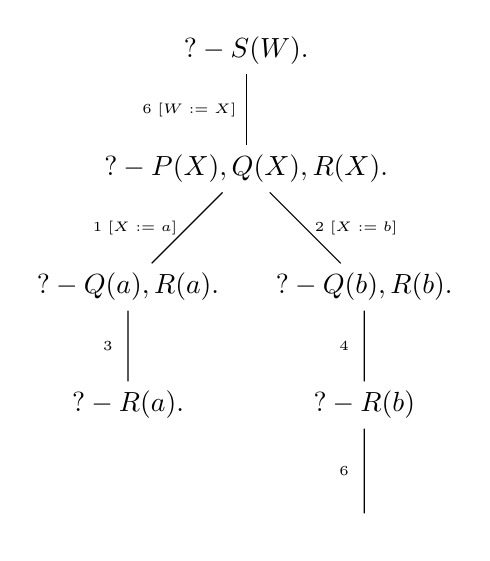
\begin{tikzpicture}
  \tikzstyle{level 1}=[sibling distance=25mm]
  \tikzstyle{level 2}=[sibling distance=30mm]
 
  \node {$?-S(W).$} 
  child { node {$?-P(X),Q(X),R(X).$}
      child {node {$?-Q(a),R(a).$}
	child { node {$?-R(a).$} edge from parent node [left] {\tiny $3 \;$} } edge from parent node [left] {\tiny $1 \; [X:=a]$}} 
      child {node {$?-Q(b),R(b).$} 
	child {node {$?-R(b)$} 
		child { node {$\cv$} edge from parent node [left] {\tiny $6 \;$} }  edge from parent node [left] {\tiny $4 \;$}  } edge from parent node [right] {\tiny $ 2 \; [X:=b]$}}
     edge from parent node [left] {\tiny $6 \;[W:=X]$} };
 \end{tikzpicture}
\caption{Árbol SLD para la meta $?.-S(W)$.}
\end{minipage}
\hspace{1.5cm}
\begin{minipage}{.4\textwidth}
\centering
 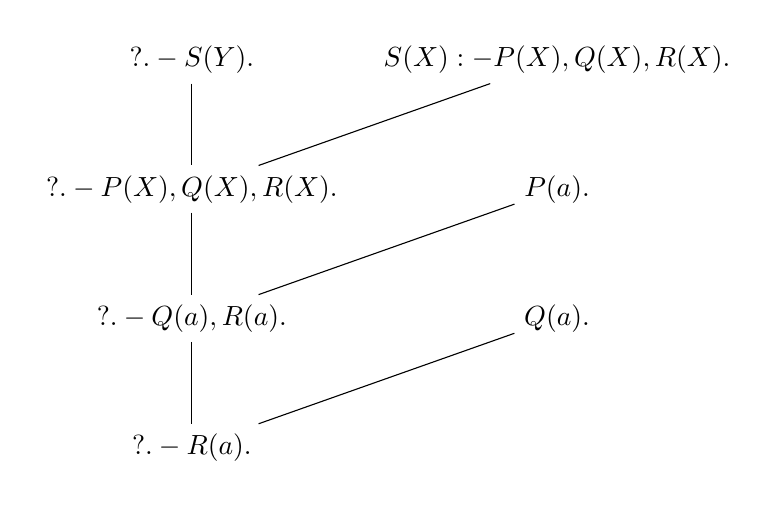
\begin{tikzpicture}
  \matrix (m) [matrix of math nodes, row sep=3em,
    column sep=1em]{
    ?.-S(Y).&  S(X):-P(X),Q(X),R(X). \\
     ?.-P(X),Q(X),R(X).& P(a). \\
    ?.-Q(a),R(a).& Q(a).  \\
    ?.- R(a). &  \\};
  \path[-]
    (m-1-1) edge (m-2-1) 
    (m-1-2) edge (m-2-1)
    (m-2-1) edge (m-3-1)
    (m-2-2) edge (m-3-1)
    (m-3-1) edge (m-4-1)
    (m-3-2) edge (m-4-1);
\end{tikzpicture}
\caption{SLD derivación para $?.- S(Y)$.}
\end{minipage}
\end{figure}

\newpage
\begin{tiny}
\begin{figure}[h!]
\centering
 \begin{tikzpicture}
  \matrix (m) [matrix of math nodes, row sep=3em,
    column sep=1em]{
    ?.-S(Y).&  S(X):-P(X),Q(X),R(X). \\
     ?.-P(X),Q(X),R(X).& P(b). \\
    ?.-Q(b),R(b).& Q(b).  \\
    ?.- R(b). & R(b).  \\
    \cv & \\};
  \path[-]
    (m-1-1) edge (m-2-1) 
    (m-1-2) edge (m-2-1)
    (m-2-1) edge (m-3-1)
    (m-2-2) edge (m-3-1)
    (m-3-1) edge (m-4-1)
    (m-3-2) edge (m-4-1)
    (m-4-1) edge (m-5-1)
    (m-4-2) edge (m-5-1);
\end{tikzpicture}
\caption{SLD refutación para $?.- S(Y).$}
\end{figure}
\end{tiny}
\eeje



\section{Sem\'antica de programas l\'ogicos}

Una parte importante de cada paradigma de programaci\'on es la
sem\'antica, por medio de la cual se le da significado a un programa,
situaci\'on que nos permite describir formalmente lo que \'este calcula.
Al inicio de esta nota mencionamos una ventaja de la programación declarativa: 
la elegancia matem\'atica resultado de la descripci\'on del programa mediante 
enunciados precisos, as\'i el significado del programa es claro y facilita su 
verificaci\'on.

\medskip

En esta secci\'on trataremos brevemente con dos clases de sem\'antica para 
programas l\'ogicos: la declarativa y la procedimental u operacional.


Comencemos observando que una cl\'ausula \verb=P :- Q1,Q2,...,Qn= de 
{\pl} tiene una interpretaci\'on declarativa y una interpretaci\'on 
procedimental:
\bi
 \item Declarativa: $P$ es v\'alida si $Q_1$ y $Q_2$ y $\ldots$ y
  $Q_n$ son v\'alidas.\\
  La interpretaci\'on declarativa permite discutir la correctud de
    la cl\'ausula.
 \item Operacional: Para ejecutar (probar) $P$ basta ejecutar $Q_1$ y $Q_2$ y 
  $\ldots$ y $Q_n$. \\
  La interpretaci\'on operacional permite considerar a la cl\'ausula como 
  la definici\'on de un proceso. Esta sem\'antica Se genera con la     
  ejecuci\'on del programa mediante las estrategias de control del int\'erprete 
  de {\pl}.
\ei

Una pregunta importante es si ambas interpretaciones generan la misma
informaci\'on, para contestarla necesitamos hablar del concepto de
respuesta de manera formal.

\defin{[Respuesta] Sean $\P$ un programa l\'ogico y $G=\meta G_1,\ldots,G_m$ una
  meta. Una respuesta para $\P\cup\{G\}$ es una sustituci\'on $\sigma$ tal que
  $Var(G_1)\cup\ldots\cup Var(G_m)\inc\mathsf{dom}(\sigma)$, es decir una
  sustituci\'on que incluye a las variables de $G$.
}

\defin{[Respuesta correcta] Decimos que una respuesta 
$\sigma$ para $\P\cup\{G\}$ es correcta si $\P\models G_i\sigma$ para toda
$1\leq i\leq m$, o equivalentemente si $\fa\P\models
\fa\big((G_1\land\ldots\land G_m)\sigma\big)$.
}

Recordemos que $\fa\vp$ denota a la cerradura universal de $\vp$ obtenida 
cuantificando universalmente todas las variables libres de $\vp$. 
An\'alogamente $\fa\P$ se obtiene de  $\P$ al cuantificar universalmente todas 
las variables de cada una de sus cl\'ausulas. Intuitivamente una respuesta
correcta para $\P\cup\{G\}$ corresponde a una consecuencia l\'ogica
particular del programa, y es entonces una significado declarativo del
programa. 

\beje Consid\'erese el programa
\[
\P=\{mq(0,suc(X)),\;mq(suc(Y),suc(X)\impp
mq(Y,X)\}.
\] 
Entonces $\sigma=[Y:=suc(suc(0))]$ es una respuesta
correcta para $?-mq(0,Y)$ pues 
\[
\fa\P\models mq(0,Y)[Y:=suc(suc(0))]
\]
\eeje

\defin{[Respuesta computada]Sean $\P$ un programa l\'ogico y $G$ una meta. Una 
sustituci\'on $\sigma$ es una respuesta computada para $\P\cup\{G\}$ si y 
s\'olo si existe una rama de \'exito en el \'arbol de SLD-resoluci\'on (o 
\'arbol de b\'usqueda) de longitud $n$ con unificadores m\'as generales
  $\mu_0,\ldots,\mu_{n-1}$ de tal forma que 
  $\sigma=\restr{\mu_0\mu_1\ldots\mu_{n-1}}{_{Var(G)}}$
}

Es decir $\sigma$ es una respuesta computada para $\P\cup\{G\}$ si y
s\'olo si $\sigma$ es la restricci\'on de la composici\'on de los unificadores 
de una rama de \'exito en el \'arbol de SLD-resoluci\'on para $\P\cup\{G\}$.

Intuitivamente una respuesta computada corresponde al resultado del proceso de 
inferencia por parte del sistema. Las respuestas computadas son aquellas que el 
int\'erprete de {\pl} devuelve al usuario. 

\beje
Si $\P=\{p(a),\;p(b),\;q(a),\;r(f(X))\impp p(X),q(X)\}$ entonces
tenemos la siguiente rama de \'exito en el \'arbol de SLD-resoluci\'on para la 
meta $G=\meta r(X)$:

\begin{small}
\begin{minipage}{.5\textwidth}
 \centering
 \[
 \begin{array}{rll}
  1. & p(a). & Hip. \\
  2. & p(b) & Hip. \\
  3. & q(a). & Hip. \\ 
  4. & r(f(Y))\impp p(Y),q(Y). & Hip.\\
  5. & \meta r(X) &Meta \\
  6. & \meta p(Y),q(Y) & SLDRes(4,5,[X:=f(Y)]) \\
  7. & \meta q(a)  & SLDRes(6,1,[Y:=a])\\
  8. & \cv. & SLDRes(3,7) 
 \end{array}
\]
\end{minipage}
\begin{minipage}{.5\textwidth}
\centering
  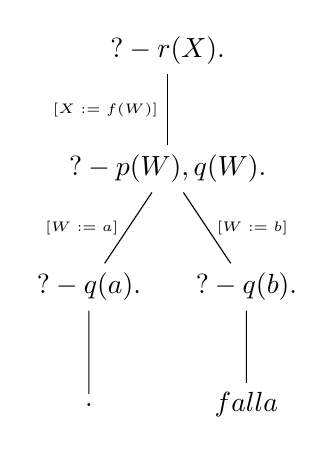
\begin{tikzpicture}
  \tikzstyle{level 1}=[sibling distance=35mm]
  \tikzstyle{level 2}=[sibling distance=20mm]
 
  \node {$?-r(X).$} 
  child { node {$?-p(W),q(W).$}
      child {node {$?-q(a).$}
	child { node {$\cv.$}} edge from parent node [left] {\tiny $[W:=a]$}} 
      child {node {$?-q(b).$} 
	child {node {$falla$}} edge from parent node [right] {\tiny $[W:=b]$}}
     edge from parent node [left] {\tiny $[X:=f(W)]$} };
 \end{tikzpicture}
\end{minipage}
\end{small}

La composici\'on de los unificadores es $[X:=f(a),Y:=a]$ de manera que 
la sustituci\'on $[X:=f(a)]$ es una respuesta computada para
$\P\cup\{\meta r(X)\}$.
\eeje

El significado de un programa l\'ogico se debe dar mediante sus respuestas, 
intuitivamente el significado es el conjunto de respuestas. Por ejemplo el 
siguiente programa $\mathbb{P}$, implementa la b\'usqueda de caminos en una 
gr\'afica:

\begin{alltt}
edge(a,b).
edge(b,c).
edge(b,d).
edge(c,d).
edge(e,f)
path(X,X).
path(X,Y) :- edge(X,Z),path(Z,Y).
\end{alltt}

De manera que el significado intensional de $\mathbb{P}$ es el conjunto de 
todos los caminos posibles (especificando todo los v\'ertices del camino) en la 
gr\'afica. Pero recordemos que la programaci\'on l\'ogica tiene un uso no 
est\'andar, por ejemplo el programa para concatenar dos listas, sirve tambi\'en 
para descomponer una lista en dos partes. Por lo que con esta definici\'on 
informal no es tan claro cu\'al es el significado. M\'as a\'un, dado un 
programa l\'ogico $\mathbb{P}$, podemos asignarle dos significados:
\begin{itemize}
 \item Significado declarativo: 
  el significado de un programa l\'ogico $\mathbb{P}$ es el conjunto de todas 
  las consecuencias l\'ogicas del programa, noci\'on asociada a la de respuesta 
  correctas.
 \item Significado operacional: 
  el significado de un programa l\'ogico $\mathbb{P}$ es el conjunto de todas 
  los \'exitos del programa, noci\'on asociada a la de respuesta computada.
\end{itemize}

Por supuesto que el significado deber\'ia ser \'unico,  pero no es claro que 
las dos nociones reci\'en enunciadas sean equivalentes. De los ejemplos 
anteriores se observa que una respuesta correcta tambi\'en es una respuesta 
computada y viceversa, ?`es esto v\'alido en general?, es decir ?`Toda
respuesta correcta puede computarse? y ?`Toda respuesta computada es
correcta? esto ayudar\'a a probar que las dos sem\'anticas coinciden.  \\
Resulta que en efecto ambos conceptos resultan equivalentes de cierta manera. 
Los enunciados formales para esta equivalencia, as\'i como su demostraci\'on 
requieren de conceptos como los modelos de Herbrand o sint\'acticos.
%M�s a�n, los dos conceptos de sem�ntica son satisfactorios desde el punto de 
% vista matem�tico pero no desde la perspectiva computacional, donde no nos 
% conformamos con conocer la definici\'on sino que requerimos en la medida de 
% lo posible de un algoritmo para calcularla. 



\end{document}
